\documentclass[12pt,fleqn]{article}
\setlength{\parindent}{0pt}
\usepackage{graphicx}
\usepackage{cancel}
\usepackage{listings}
\usepackage[latin5]{inputenc}
\usepackage{color}
\setlength{\parskip}{8pt}
\setlength{\parsep}{0pt}
\setlength{\headsep}{0pt}
\setlength{\topskip}{0pt}
\setlength{\topmargin}{0pt}
\setlength{\topsep}{0pt}
\setlength{\partopsep}{0pt}
\setlength{\mathindent}{0cm}

\begin{document}
Ders 17

Onceki derste 

\[ \int \int (1-x^2-y^2) dA \]

\[ x^2+y^2 \le 1 \]

\[ x,y \ge 0 \]

entegralini hesapladik, fakat kullandigimiz yontem biraz karmasikliga yol
acti. Daha iyi bir yontem kutupsal forma gecmektir. 

Hatirlarsak $x,y$ kordinat sisteminde cift entegral icin entegrasyon
alanini yatay, dikey sekilde parcalara ayirmistik, $dA = dy \ dx$ haline
gelmisti. Kutupsal formda 

\[ \int \int  ... \ dr \ d\theta\]

seklinde bir form olur, once $r$ uzerinden entegrasyon en kolayi. Bu
demektir ki $\theta$'yi sabitleriz, ve $r$ uzerinde hareket ederiz. 

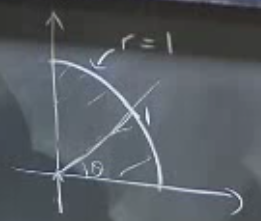
\includegraphics[height=3cm]{17_1.png}

Birim disk orneginde bu hareket basit, $r=0$'dan baslanir, ve 1 degerine
gelinceye kadar hareket edilir. $\theta$ icin 0'dan baslanir, ustteki alana
gore, $\pi/2$'ya gelinceye kadar hareket edilir. Sinirlar soyle olur:

\[ \int_0^{\pi/2} \int_0^1  ... \ dr \ d\theta\]

Fakat, dikkat, bu onemli bir nokta, $dA$ buyuklugu $dr \ d\theta$'ya esit
{\em degildir}. 

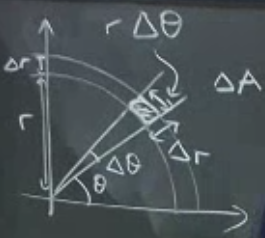
\includegraphics[height=3cm]{17_2.png}

Ustteki resimdeki ici karalanmis ufak dikdortgeni dusunelim, dikdortgenin
kenarlarindan biri biraz egimlidir (cemberin parcasi oldugu icin) fakat
kenarlar kuculdukce bu ufak alan dikdortgen olarak gorulebilir. Neyse,
kenarlarin biri $\Delta r$ (bu kolay), digeri? Oteki kenar $\Delta \theta$
degil, cunku o kenar cemberin bir parcasi, o zaman $r \ \Delta \theta$.

Bu demektir ki kenarlari sonsuz kuculttugumuz zamanda bile 

\[ dA = r \ dr \ d\theta \]

olacak. 








\end{document}
